\chapter{Sensor Fusion}
Nei sistemi in cui \`e richiesta un'alta \emph{reliability} delle misure, l'informazione fornita dai singoli sensori non \`e sufficiente. In questi casi \`e raccomandato l'utilizzo di un insieme di sensori in contemporanea.\\*
\section{Panoramica}
In generale, un algoritmo SFA viene utilizzato per stimare lo stato di un sistema dinamico in un ambiente caratterizzato da \emph{rumore}.
\subsection{Sistemi Dinamici}
Un sistema dinamico \`e una modellazione matematica di un processo che evolve nel tempo, la cui evoluzione \`e descritta attraverso un sistema di equazioni differenziali o alle differenze, nel caso esso si evolva rispettivamente a tempo continuo o a tempo discreto.\\*
Sia $S$ l'insieme dei possibili stati che il sistema pu\`o assumere, e sia $m = |S|$ la dimensione dello spazio degli stati.\\*
Senza perdere in generalit\`a, si possono formalizzare questi due tipi di sistemi dinamici come:
$$
y'(t) = f(t,y(t)),\;t\ge 0\;\;\;\;(1)
$$
Con $y(0) \in \mathbb{R}^m$ condizione iniziale nota, e:
$$
y_{n+1} = f(n,y_n),\;n = 0,1,\dots\;\;\;\;(2)
$$
con al solito $y_0 \in \mathbb{R}^m$ condizione iniziale nota.\\*
Ricavare lo stato del sistema dinamico per un certo istante $t$, o $n$, equivale a risolvere le equazioni cui sopra e valutarne la traiettoria soluzione in $t$ o in $n$.\\*
Un semplice sistema dinamico \`e rappresentato da un punto materiale che si muove con una accelerazione costante $$\mathbf{a} = a\mathbf{k}$$ dove $\mathbf{k}$ \`e un qualunque versore della base canonica di $\mathbb{R}^3$.\\*
Supponendo che il punto si muova con velocit\`a iniziale $\mathbf{z'}(0) = v_0\mathbf{k}$ nota e inizi il moto da una coordinata $\mathbf z(0) = z_0\mathbf{k}$ nota, si ha:
$$
z''(t) = a\;\;\;\;(3)
$$
$$
z'(t) = \int{a dt} = a t + v_0
$$
$$
z(t) = \int(a t + v_0)dt = \frac{1}{2} at^2 +  v_0 t + z_0
$$
L'equazione $z(t)$ descrive completamente la traiettoria di moto del punto materiale, mentre $z'(t)$ descrive completamente la traiettoria della velocit\`a del punto durante il suo moto.
\subsection{Misure e Rumore}
In questo semplice esempio, viene fatta l'assunzione di conoscere a priori il valore esatto di $a$, di $v_0$ e di $z_0$.\\*
Nella pratica, per misurare l'accelerazione $a$ \`e necessario uno strumento denominato \emph{accelerometro}, il quale produrr\`a delle misure giocoforza affette da errori casuali. Si supponga di sostituire $a$ nell'equazione $z(t)$ con una sua perturbazione $\tilde{a} = a + \varepsilon$ dove $\varepsilon$ \`e una variazione casuale della misura data dal \emph{rumore} che caratterizza qualsiasi processo di misura. Si pu\'o supporre $Var(\varepsilon) = 0$ e considerare, ai fini di questa trattazione, $\varepsilon$ come un valore costante; in realt\`a $\varepsilon$ \`e una variable casuale a varianza generalmente non nulla. Si suppongano inoltre $v_0 = z_0 = 0$ per comodit\`a di calcolo:
$$
z(t) = \frac{1}{2} \tilde{a} t^2 = \frac{1}{2}(a + \varepsilon) t^2 = \frac{1}{2} \left(at^2 + \varepsilon t^2\right)
$$
Si nota immediatamente che la variazione della misura $z(t)$ data da $\varepsilon$ aumenta con il quadrato del tempo.\\*
\begin{figure}[h]
	\centering
	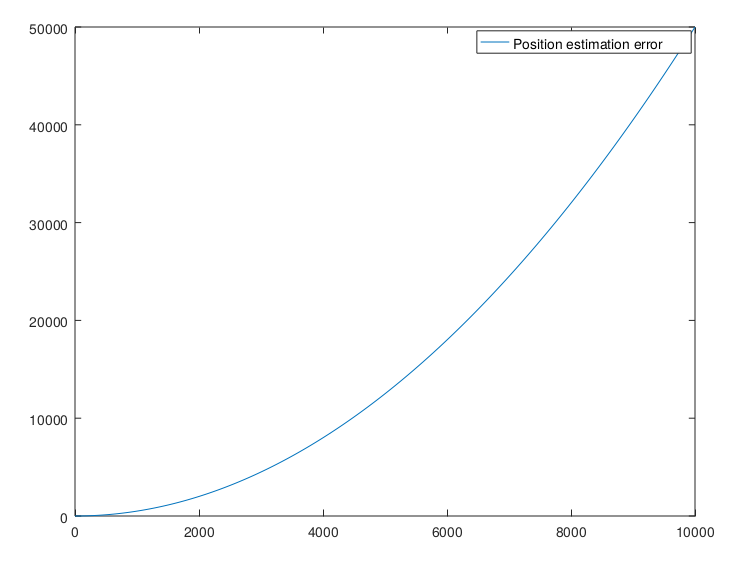
\includegraphics[scale=0.5]{img/errormeas}
	\caption{Grafico dell' errore di stima della posizione con $a = 10^0, \varepsilon = 10^{-3}$}
	\label{fig:errormeas}
\end{figure}\newpage
Il sistema dinamico individuato in $(3)$, \`e una tipologia di sistema dinamico caratterizzato da assenza di \emph{rumore di processo}: fatta assunzione di conoscere esattamente il valore di $a$, la doppia integrazione di $(3)$ rispetto al tempo fornisce una descrizione esatta e deterministica della dinamica del sistema: la traiettoria sar\`a \emph{esattamente} quella individuata dalla soluzione.\\*
Alcuni processi tuttavia evolvono in parte stocasticamente per loro natura, e questa natura stocastica insita nel processo viene chiamata \emph{rumore di processo}. Si conclude pertanto che non solamente le misurazioni sono affette da rumore, ma anche il processo evolutivo stesso pu\`o essere affetto da rumore stocastico intrinseco.
\newpage
\section{I Filtri di Kalman}
Un Filtro di Kalman, o in inglese \emph{Kalman Filter} (KF), \`e un modello di SFA progettato appositamente per risolvere o rendere trascurabile il problema del rumore.\\*
Esso \`e, da un punto di vista statistico, uno \emph{stimatore} dello stato di un sistema dinamico caratterizzato da rumore.
\subsection{Premesse statistiche}
\`E opportuno fissare la notazione che sar\`a usata nelle discussioni che seguiranno.\\*
Siano $X_1,\dots,X_N$ $N$ variabili casuali.\\*
Si ha che ciascuna $X_i$ \`e caratterizzata da una distribuzione di probabilit\`a:
$$
p_{X_i} = \{p_j:P(X_i = j) = p_j\},\;\;\;\;i = 1,\dots,N
$$
Per una data variabile casuale $X$, con distribuzione di probabilit\`a $p_X$, si definisce la \emph{media}, o \emph{valore atteso}, di $X$ come:
$$
\mathbb{E}(X) = \sum_{i=1}^{+\infty} X_i p_{X_i} = \mu_X
$$
Si definisce \emph{varianza} di $X$, la quantit\`a:
$$
Var(X) = \mathbb{E}[(X-\mu_X)]^2 = \sum_{i=1}^{+\infty} (X_i - \mu_X)^2p_{X_i} = \sigma^2_X
$$
Date due variabili casuali, siano esse $X$ e $Y$, definite sullo stesso insieme di cardinalit\`a $M$, si chiama \emph{covarianza} di $X,Y$ la seguente quantit\`a:
$$
cov(X,Y) = \frac{1}{M}\sum_{i=1}^M (X-\mathbb{E}(X))(Y-\mathbb{E}(Y)) = \sigma_{XY}
$$
Si osservi che :
$$
cov(X,X) =  \frac{1}{M}\sum_{i=1}^M (X-\mathbb{E}(X))(X-\mathbb{E}(X)) =  \frac{1}{M}\sum_{i=1}^M (X-\mathbb{E}(X))^2 = \sigma^2_X
$$
Per una variabile aleatoria multivariata, quale una distribuzione di probabilit\`a congiunta su $N$ variabili casuali, siano esse $X_1,\dots,X_N$, si definisce la matrice di \emph{varianza-covarianza}, o semplicemente matrice di \emph{covarianza}, la seguente matrice quadrata $N$\texttt{x}$N$:
$$
\Sigma = \left(\begin{matrix}
cov(X_1,X_1) && cov(X_1,X_2) && \dots && cov(X_1,X_N) \\
\vdots && \vdots && \vdots \\
cov(X_N,X_1) && cov(X_N, X_2) && \dots && cov(X_N,X_N)
\end{matrix}\right) 
$$
$$
 = \left(\begin{matrix}
\sigma^2_{X_1} && \sigma_{X_1,X_2} && \dots && \sigma_{X_1,X_N} \\
\vdots && \vdots && \vdots \\
\sigma_{X_N,X_1} && \sigma_{X_N, X_2} && \dots && \sigma^2_{X_N}
\end{matrix}\right)
$$
Si osserva che $\Sigma$ \`e una matrice \emph{simmetrica} per la propriet\`a commutativa del prodotto:
$$
cov(X,Y) = \frac{1}{M}\sum_{i=1}^M (X-\mathbb{E}(X))(Y-\mathbb{E}(Y)) = 
$$
$$
 = \frac{1}{M}\sum_{i=1}^M (Y-\mathbb{E}(Y))(X-\mathbb{E}(X)) = cov(Y,X)
$$
\subsection{Filtro di Kalman Lineare}
I KF sono comunemente basati su sistemi dinamici \emph{lineari} a tempo discreto, tuttavia i fenomeni reali sono raramente lineari. Un modello lineare \`e spesso un'approssimazione di un modello pi\`u complesso.\\*
Nel dominio applicativo in cui si colloca la Tesi, ossia quello del posizionamento ferroviario, occorre utilizzare una generalizzazione al caso non-lineare dei Filtri di Kalman standard: il Filtro di Kalman Esteso (CITARE PAPER QUA). Pper ragioni di semplicit\`a, in questo capitolo viene esposto il principio base del funzionamento di un semplice KF llineare.
\subsubsection{Definizione del problema}
Si consideri il seguente sistema dinamico lineare discreto:
$$
\begin{cases}
\mathbf x_k = A \mathbf x_{k-1} + B \mathbf u_k + \mathbf w_k \\
\mathbf y_k = C \mathbf x_k + \mathbf v_k
\end{cases}
$$
In cui i vettori $\mathbf w_k$ e $\mathbf v_k$ rappresentano rispettivamente il rumore di processo e il rumore di misura. Si assumono \emph{congiuntamente gaussiani}, indipendenti e con matrici di covarianza $Q,R$ rispettivamente.\\*
Il vettore $\mathbf y_k$ rappresenta il vettore di misurazioni campionate all'istante $k$, mentre il vettore $\mathbf x_k$ rappresenta lo stato del sistema all'istante $k$.\\*
Le matrici $A$ e $B$ descrivono la dinamica del modello e si assumono note a priori, pena l'introduzione di errori sistematici, mentre la matrice $C$ descrive la dinamica del processo di misura.